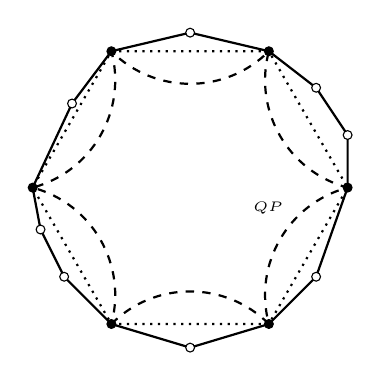
\begin{tikzpicture}[scale=2]
    % outer local marginal polytope
    \draw[thick]
    (0,0) -- (0.5,-0.15) -- (1,0) -- (1.3,0.3) --
    (1.5,0.866) -- (1.5,1.2) -- (1.3,1.5) -- (1,1.732) -- (0.5,1.85) -- (0,1.732) --
    (-0.25,1.4) -- (-0.5,0.866) -- (-0.45,0.6) -- (-0.3,0.3) -- (0,0);

    % marginal polytope
    \draw[thick, dotted]
    (0,0) -- (1,0) --
    (1.5,0.866) -- (1,1.732) -- (0,1.732) -- (-0.5,0.866) -- cycle;

    % inner QP approximation
    \draw[thick,out=45,in=135,relative, dashed]
    (0,0) to (1,0) to
    (1.5,0.866) to (1,1.732) to (0,1.732) to (-0.5,0.866) to (0,0);

    % integer solutions
    \filldraw (0,0) circle (0.8pt);
    \filldraw (1,0) circle (0.8pt);
    \filldraw (1.5,0.866) circle (0.8pt);
    \filldraw (1,1.732) circle (0.8pt);
    \filldraw (0,1.732) circle (0.8pt);
    \filldraw (-0.5,0.866) circle (0.8pt);

    % fractional solutions
    \filldraw[fill=white] (0.5,-0.15) circle (0.8pt);
    \filldraw[fill=white] (1.3,0.3) circle (0.8pt);
    \filldraw[fill=white] (1.5,1.2) circle (0.8pt);
    \filldraw[fill=white] (1.3,1.5) circle (0.8pt);
    \filldraw[fill=white] (0.5,1.85) circle (0.8pt);
    \filldraw[fill=white] (-0.25,1.4) circle (0.8pt);
    \filldraw[fill=white] (-0.45,0.6) circle (0.8pt);
    \filldraw[fill=white] (-0.3,0.3) circle (0.8pt);

    \node (lp) at (1.5,1.5) {\scriptsize$\localmarginalpolytope_{\gmgraph}$};
    \node (ip) at (0.5,0.1) {\scriptsize$\marginalpolytope$};
    \node (qp) at (1,0.7) {\scriptsize$\localmarginalpolytope_{\gmgraph}^{QP}$};
\end{tikzpicture}
